% chktex-file 4:
%! TEX root = ./main.tex
% chktex-file 1
% chktex-file 36

\begin{Aufgabe}{2}
	Lies an den markierten Stellen (A, B, C und D) des Zahlenstrahls die Zahlen ab.

	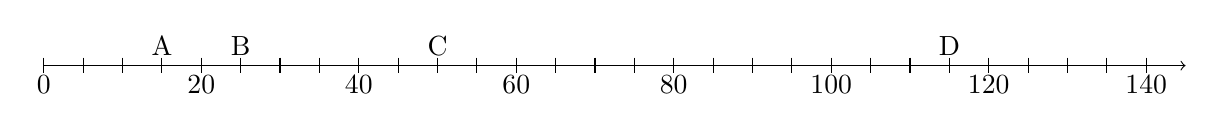
\begin{tikzpicture}
	  \draw[->] (0,0) -- (14.5,0);
	  \foreach \x in {0, 0.5, ..., 14} % chktex 12
	  \draw (\x,0.1) -- (\x,-0.1);

	  \foreach \x in {0, 20, 40, 60, 80, 100, 120, 140}
	  \node[below] at ({\x/10}, 0) {\x};

	  \node[above] at (1.5, 0) {A};
	  \node[above] at (2.5, 0) {B};
	  \node[above] at (5.0, 0) {C};
	  \node[above] at (11.5, 0) {D};
	\end{tikzpicture}
\end{Aufgabe}

\begin{Loesung}
	A:\@15; \HalberPunkt{}\hspace{.3cm} B:\@25; \HalberPunkt{}\hspace{.3cm} C:50; \HalberPunkt{}\hspace{.3cm} D:\@115 \HalberPunkt{}
\end{Loesung}

\begin{Aufgabe}{2}
	\begin{tasks}
		\task Zeichne einen Zahlenstrahl von 0 bis 12. Wähle \SI{1}{\centi\meter} für den Abstand von 0 bis 1.
		\task Markiere auf dem Zahlenstrahl alle Zahlen, die kleiner als 9 und größer als 3 sind.
	\end{tasks}
\end{Aufgabe}

\begin{Loesung}
	\begin{tasks}
		\task Beschriftung \HalberPunkt{}. Zahlen von 0 bis 12 abgebildet \HalberPunkt{}
		\task Zahlen 4, 5, 6, 7 und 8 sind markiert \Punkt{}
	\end{tasks}
\end{Loesung}

\begin{Aufgabe}{2}
	Zeichne einen Zahlenstrahl, auf dem die Zahlen 102, 112, 108 und 107 gut zu sehen sind.
\end{Aufgabe}

\begin{Loesung}
	\begin{itemize}
		\item[\Punkt{}] Übersichtlich und korrekt gezeichneter Zahlenstrahl.
		\item[\Punkt{}] Die Zahlen 102, 107, 108 und 112 liegen auf einem Kästchenstrich und sind beschriftet.
	\end{itemize}
\end{Loesung}
